\documentclass{article}

\usepackage{ctex}
\usepackage{geometry}
\usepackage{longtable}
\usepackage{graphicx}
\usepackage{listings}
\usepackage{xcolor}
\usepackage{float}
\usepackage{amsmath}

\lstset{
    basicstyle          =   \small,          % 基本代码风格
    keywordstyle        =   \bfseries,          % 关键字风格
    commentstyle        =   \rmfamily\itshape,  % 注释的风格,斜体
    stringstyle         =   \ttfamily,  % 字符串风格
    flexiblecolumns,                % 别问为什么,加上这个
    numbers             =   left,   % 行号的位置在左边
    showspaces          =   false,  % 是否显示空格,显示了有点乱,所以不现实了
    numberstyle         =   \zihao{-5}\ttfamily,    % 行号的样式,小五号,tt等宽字体
    showstringspaces    =   false,
    captionpos          =   t,      % 这段代码的名字所呈现的位置,t指的是top上面
    frame               =   lrtb,   % 显示边框
    breaklines,
}


\lstdefinestyle{C}{
    language        =   C,
    basicstyle      =   \zihao{-5}\ttfamily,
    numberstyle     =   \zihao{-5}\ttfamily,
    keywordstyle    =   \color{blue},
    keywordstyle    =   [2] \color{teal},
    stringstyle     =   \color{magenta},
    commentstyle    =   \color{red}\ttfamily,
    breaklines      =   true,   % 自动换行,建议不要写太长的行
    columns         =   fixed,  % 如果不加这一句,字间距就不固定,很丑,必须加
    basewidth       =   0.5em,
}

\geometry{scale=0.8}

\title{C语言教程讲义}
\author{Potato}

\begin{document}

\setcounter{section}{-1}

\maketitle

本文件编译于\today

\section{计算机基础知识与计算机语言概述}
\section{标准输出和变量}

\subsection{printf函数}

打开visual studio,在“源文件”上右键,点击“添加”->“新建项”,创建一个叫main.c的文件,在其中输入

\begin{lstlisting}[language=C]
    #include <stdio.h>
    
    int main() {
        printf("Hello World!");

        return 0;
    }
\end{lstlisting}

点击“本地Windows调试器”,将会出现类似于这样的界面

\begin{figure}[H]
    \centering
    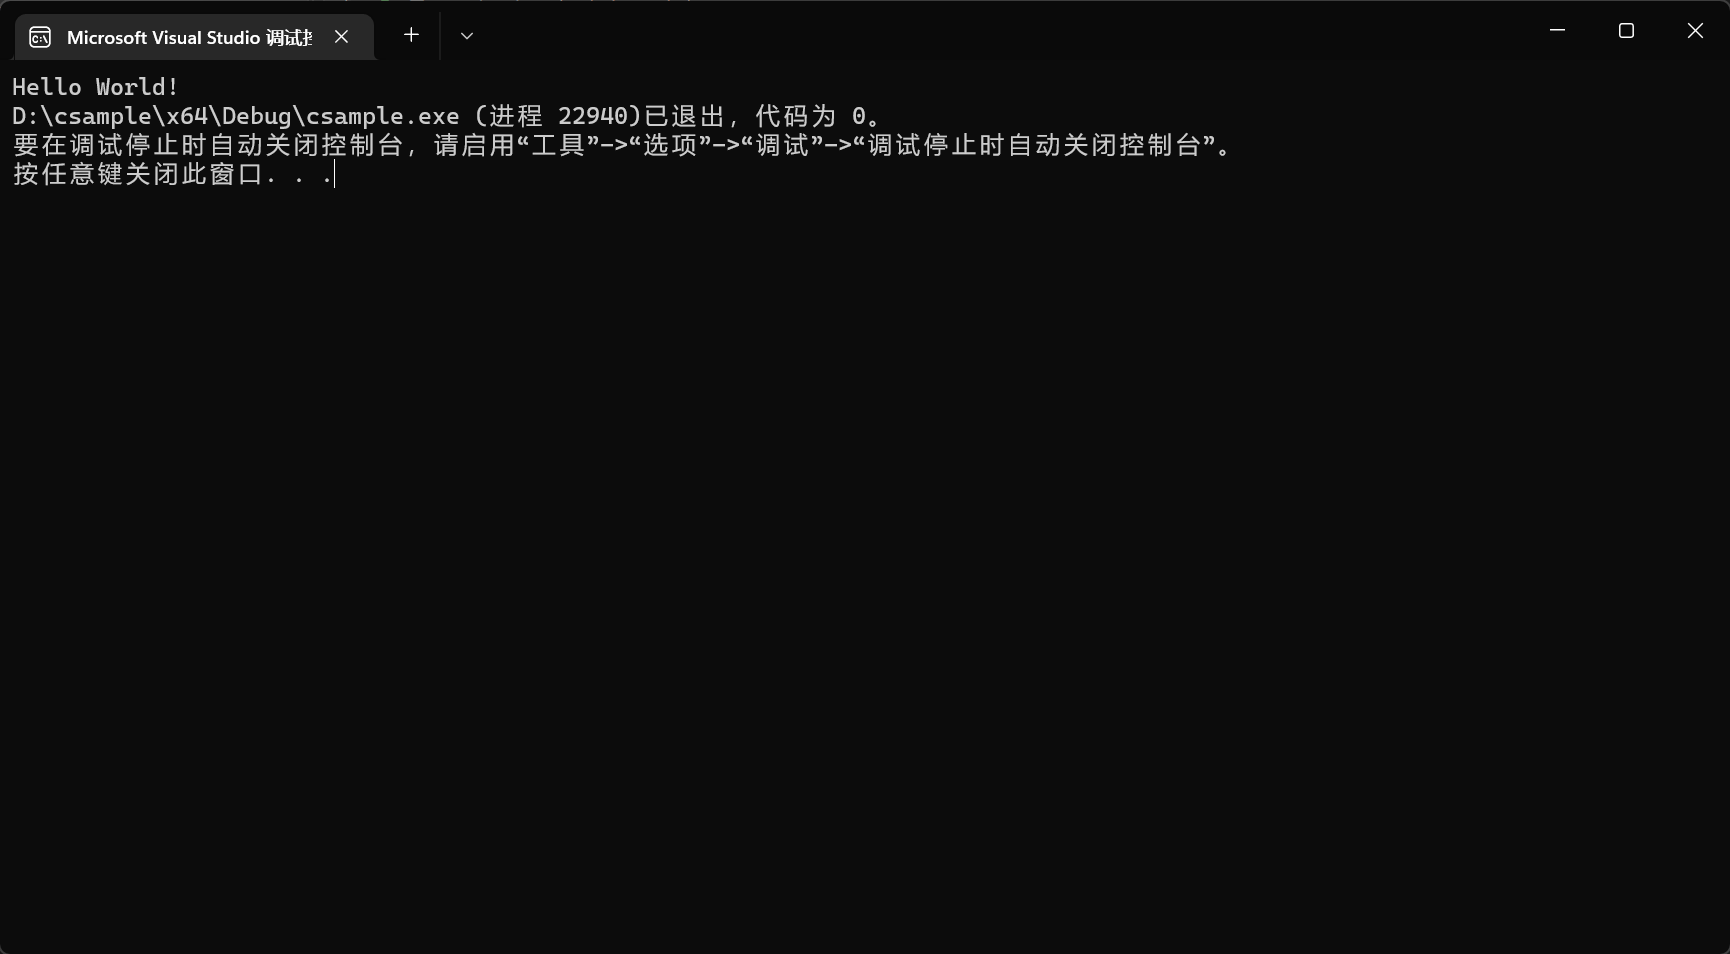
\includegraphics[width=0.8\textwidth, height=0.4\textheight]{images/1HelloWorld结果.png}
\end{figure}

恭喜你写出了你的第一段代码。计算机领域有一个传统:刚入门编程的人的第一段代码一定要是Hello World,这是我们对无垠的计算机世界打的招呼。这个黑乎乎的界面叫做终端(这里不做关于终端、shell等的详细区分),我们以后会常常和它打交道。

我们发现,我们写在printf的引号内的内容会被打印出来(顾名思义,printf就是print function嘛),因此我们可以多写几个printf(不要忘了每行最后的英文分号),如

\begin{lstlisting}[language=C]
    #include <stdio.h>
    
    int main() {
        printf("Hello World!");
        printf("Potato");

        return 0;
    }
\end{lstlisting}

运行代码,我们观察到Hello World和Potato输出在了同一行。我们想要的是这二者各自占一行,那就需要在Hello World!后加一个换行符,也即$\backslash$n,代码就变成了

\begin{lstlisting}[language=C]
    #include <stdio.h>
    
    int main() {
        printf("Hello World!\n");
        printf("Potato\n");

        return 0;
    }
\end{lstlisting}

这次的结果就是我们想要的了。为什么Potato也要加换行符?这是因为也许我们在其后还会添加新的printf,要是到时候忘了给Potato加换行符,不就没有实现我们想要的效果吗?为了避免以后出现不必要的问题,我们推荐每个printf后都加换行符。

由上面的代码,我们总结出了这些要点:首先,我们要想输出信息,就要将其写在printf的引号内;其次,要想换行,就需要在输出的文本最后加一个换行符$\backslash$n;另外我们还注意到,我们先输出了Hello World,再输出了Potato,也就是说,程序是按照从上到下的顺序执行的。

这是很重要的结论,所以我们使用printf输出一遍加强印象吧。于是我们写下了:

\begin{lstlisting}[language=C]
    printf("首先,我们要想输出信息,就要将其写在printf的引号内;其次,要想换行,就需要在输出的文本最后加一个换行符\n;\n");
\end{lstlisting}

我们注意到有个问题,就是第一个换行符是我们想要按照文本形式输出的,但是如果按照上面的写法,它会被用于换行而不是直接输出。为了解决这个问题,我们把代码改成这样即可:

\begin{lstlisting}[language=C]
    printf("首先,我们要想输出信息,就要将其写在printf的引号内;其次,要想换行,就需要在输出的文本最后加一个换行符\\n;\n");
\end{lstlisting}

运行结果是:

\begin{figure}[H]
    \centering
    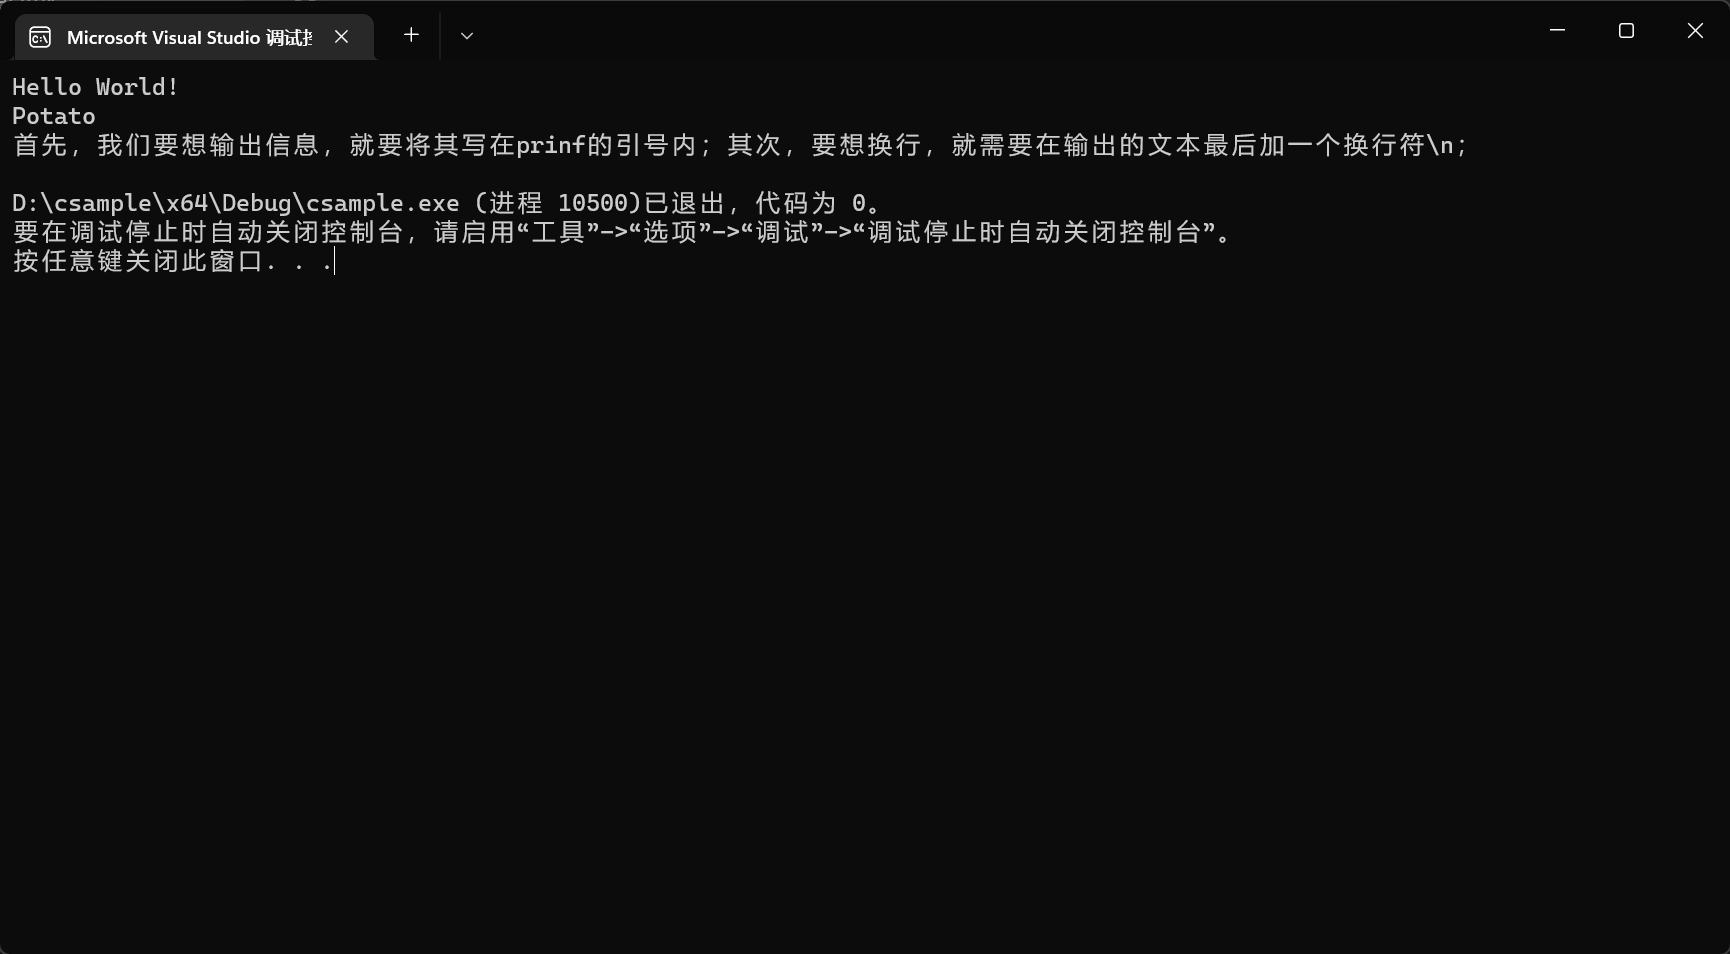
\includegraphics[width=0.8\textwidth, height=0.4\textheight]{images/1换行符输出.png}
\end{figure}

为什么会这样呢?实际上,我们输入的$\backslash$n和$\backslash{}\backslash$都叫做转义符号,用来实现一些特殊的输出效果。它的语法就是反斜杠($\backslash$)加一个字母。我们最常用的转义符号就是换行符$\backslash$n,实际上还有$\backslash$t、$\backslash$a等等。因为反斜杠会和下一个字母结合变成转义符号,所以要想输出反斜杠,就需要按照上面的例子那样使用两个反斜杠,这个转义符号的结果就是输出一个反斜杠。

\subsection{变量}

变量顾名思义,就是可以变的量。一个变量肯定要有名字,然后要有一个值。这就像是我们的考试成绩,有一个叫做“数学成绩”的变量,这次可以是120,下次可以是130。在c语言中,我们这样声明变量:$type\quad{}name$,啥意思呢,比如我们要声明数学成绩(math\_grade),那么就可以这样写

\begin{lstlisting}[language=C]
    int math_grade; 
\end{lstlisting}

这里的int是整数的意思,还有其它类型(如小数)我们之后会讲到。所以这行代码的意思就是,我们声明了一个叫做math\_grade的变量,它是一个整数。接下来就要给它赋值了,在大部分计算机语言中,赋值号都是=,比如数学成绩是120,那么就可以写

\begin{lstlisting}[language=C]
    math_grade = 120;
\end{lstlisting}

这段代码的意思就是给math\_grade赋予120这个值。也即,我们将赋值号右边的值给了左边的变量。我们强调是将右边的值赋给左边,说明了这不是数学中的等号,它不意味着左右两边相等,也不能交换左右两边的位置。

现在我们的main.c应该是这样的

\begin{lstlisting}[language=C]
    #include <stdio.h>

    int main() {
        int math_grade;
        math_grade = 120;

        return 0;
    }
\end{lstlisting}

第四行是声明变量,第五行是给变量赋值。如果我们在声明变量时就知道它要赋什么值,那么就可以把声明和赋值写在一起

\begin{lstlisting}[language=C]
    int math_grade = 120;
\end{lstlisting}

如果要同时声明多个类型一样的变量,那么可以写在一行,比如同时声明数学、语文和英语成绩:

\begin{lstlisting}[language=C]
    int math_grade, chinese_grade, english_grade;
\end{lstlisting}

不过笔者推荐每个变量单独成行,因为在最开始写代码时,我们可能由于考虑不周会选错变量类型(比如英语成绩会出现0.5分的情况,那么选择整数就不合适了),如果写在同一行会增大修改的难度,因此推荐每个变量分开声明:

\begin{lstlisting}[language=C]
    int math_grade;
    int chinese_grade;
    int english_grade;
\end{lstlisting}

那么变量的命名遵循怎样的原则呢?我们这里的命名是math\_grade,其实也可以命名成MathGrade,也可以是mathGrade,可以是拼音shuxuechengji,甚至可以是汉语的数学成绩,如果你比较懒,直接命名l这样的单字母都可以。c语言要求,变量名开头不是数字、不包含空格、标点和\%、@等符号,不是c语言关键字(后面会介绍这个概念)即可。那么我们为什么使用了math\_grade呢?

首先我们说明为什么不用汉语或者汉语拼音。一方面,由于编码不同,在你的电脑上正常显示的中文可能在别人电脑上就变成了乱码(这就是第零章要求大家切换UTF8编码的原因),这样严重影响了正常的开发和交流工作。另一方面,大家有没有发现,当你在声明好变量后,你敲下“m”时就会出现一个框,可以直接补全math\_grade,这是IDE的自动补全功能,如果使用中文就无法自动补全了。zhi yu wei shen mo bu yong pin yin, ge wei jue de zhe yang de ke du xing gao ma?

计算机语言的核心在于其逻辑而不是用了什么自然语言作为支撑,哪怕世界上第一门计算机语言是中国人发明的,计算机语言也会愈发趋向于使用字母来构成,因为这样效率更高。这样大家就可以明白那些被大肆宣扬的“汉语编程语言”的荒谬之处了,不要陷入了虚伪的爱国主义的陷阱。

我们命名的math\_grade有个特点:单词全部小写,单词之间使用下划线\_连接。这种命名方式叫做蛇形命名法(snake\_case)。至于我们上面提到的mathGrade也是一种命名法,叫做小驼峰命名法(camelCase)。命名法和一些其它规则构成了代码风格(code style),本讲义遵循Google代码规范,也推荐各位使用这套代码规范。各位在阅读此讲义时应该注意示例代码的代码风格,自己写代码时要模仿示例代码的风格。不过,如果各位是参与到他人的项目,自然是要按照他人已有的标准来写代码。

代码风格提示:变量命名使用蛇形命名,即connect\_every\_lowercase\_word\_by\_underscore

我们可以这样打印整数变量

\begin{lstlisting}[language=C]
    #include <stdio.h>

    int main() {
        int math_grade;
        math_grade = 120;

        printf("%d\n", math_grade); 

        return 0;
    }
\end{lstlisting}

运行程序,输出了120。我们目前只需要这样理解:引号内的\%d是一个占位符,引号后面的math\_grade就是用来替换占位符的。因此我们就可以实现一些更复杂的输出了,比如

\begin{lstlisting}[language=C]
    printf("数学成绩为:%d\n", math_grade); 
\end{lstlisting}

现在拓展一下,如果我们定义了数学、语文和英语三门课的成绩,也即

\begin{lstlisting}[language=C]
    int math_grade = 120;
    int chinese_grade = 100;
    int english_grade = 140;
\end{lstlisting}

如何输出呢?我们只需要写三个占位符即可,也就是

\begin{lstlisting}[language=C]
    printf("数学成绩为:%d,语文成绩为:%d,英语成绩为:%d\n", math_grade, chinese_grade, english_grade); 
\end{lstlisting}

想象一下,假如我们定义了很多变量,有数学期中成绩,数学期末成绩,语文小测成绩,语文期末成绩……我们在代码里看这么多东西就头大,所以我们希望能用自然语言给它们加上注释,便于我们理解代码。在c语言中,有两种形式的注释:单行注释和多行注释。

单行注释是两个斜杠(//),这两个斜杠之后就可以随便写字了,比如

\begin{lstlisting}[language=C]
    #include <stdio.h>

    int main() {
        int math_grade;  // 声明数学成绩
        math_grade = 120;  // 给数学成绩赋值120

        printf("%d\n", math_grade);   // 打印数学成绩
        // 单行注释也可以单独成行

        return 0;
    }
\end{lstlisting}

多行注释的语法是/* */,在这之间可以随便写字,比如

\begin{lstlisting}[language=C]
    #include <stdio.h>

    int main() {
        /*
            该程序的展示了变量的声明与赋值语法,
            以及使用printf打印整型变量的方法
        */
        int math_grade;  // 声明数学成绩
        math_grade = 120;  // 给数学成绩赋值120

        printf("%d\n", math_grade);   // 打印数学成绩

        return 0;
    }
\end{lstlisting}

需要注意的是,多行注释不能这样写

\begin{lstlisting}[language=C]
    int math_grade;  /* 声明数学成绩 
    math_grade = 120;  给数学成绩赋值 */
\end{lstlisting}

这样的话,第二段代码就被包括在了注释内,从而无法执行。

那么什么时候用单行注释,什么时候用多行注释呢?如果写注释的目的是对一行或几行代码做简单的说明,那么就用单行注释;假如注释的目的是要阐释一个复杂的原理(比如一段算法的数学原理或工程背景)或者解释一个函数(接下来会讲函数是什么)的功能,那么就应该使用多行注释。

有了变量,肯定也要有常量。在c语言中,我们使用\#define来声明常量。比如,圆周率$\pi$就是一个常量,我们可以这样在c语言中定义圆周率

\begin{lstlisting}[language=C]
    #define PI 3 
\end{lstlisting}

也即,定义常量的语法是\#define 常量名 常量的值。

我们定义圆周率是3,是一个整数,因此可以按照上文的方法将其打印出来

\begin{lstlisting}[language=C]
    #include <stdio.h>

    #define PI 3

    int main() {
        printf("圆周率的近似值是%d\n", PI);

        return 0;
    }
\end{lstlisting}

你可能觉得奇怪,为什么定义常量的语法和变量区别这么大呢?既不需要写赋值号,也不需要标明类型。实际上,\#define是一个宏,在c语言中,程序被编译运行前,会有一个叫做预处理器的程序将所有宏替换为对应的值,也就是说(在只考虑\#define宏的情况下),上面的代码经过预处理器会变成这样

\begin{lstlisting}[language=C]
    #include <stdio.h>

    int main() {
        printf("圆周率的近似值是%d\n", 3);

        return 0;
    }
\end{lstlisting}

发现了吗?我们定义的常量PI被直接替换成了它的值$3$,既然是直接替换,就相当于是写死在了程序里,没法修改,所以就是常量了。实际上,我们行首的\#include也是一个宏,它的效果和\#define类似。关于宏和预处理的知识我们在之后会学习到。

代码风格提示:命名常量,一般采用大驼峰命名法(CamelCase),也即所有单词都连在一起,每个单词的首字母大写。如CapitalizeTheFirstLetterOfEachWord

\subsection{scanf函数}

scanf函数是scan function,它用来从终端获取输入的文本。这个东西涉及到一些我们还没有学到的知识,但是我们后续的学习很难离开它,因此需要在这里对其简单介绍,我们目前不需要了解它的原理,会用就可以。

首先,打开visual stdio,在main.c中输入一段这样的代码

\begin{lstlisting}[language=C]
    #include <stdio.h>

    int main() {
        int num;  // 用于储存用户输入的数字
        printf("请输入一个整数");  // 提示用户进行输入
        scanf("%d", &num);  // 将输入的数字保存在变量num中,注意不要忘了num前的&

        printf("你输入的整数是%d", num);

        return 0;
    }
\end{lstlisting}

点击运行,出现了意料之外的情况

\begin{figure}[H]
    \centering
    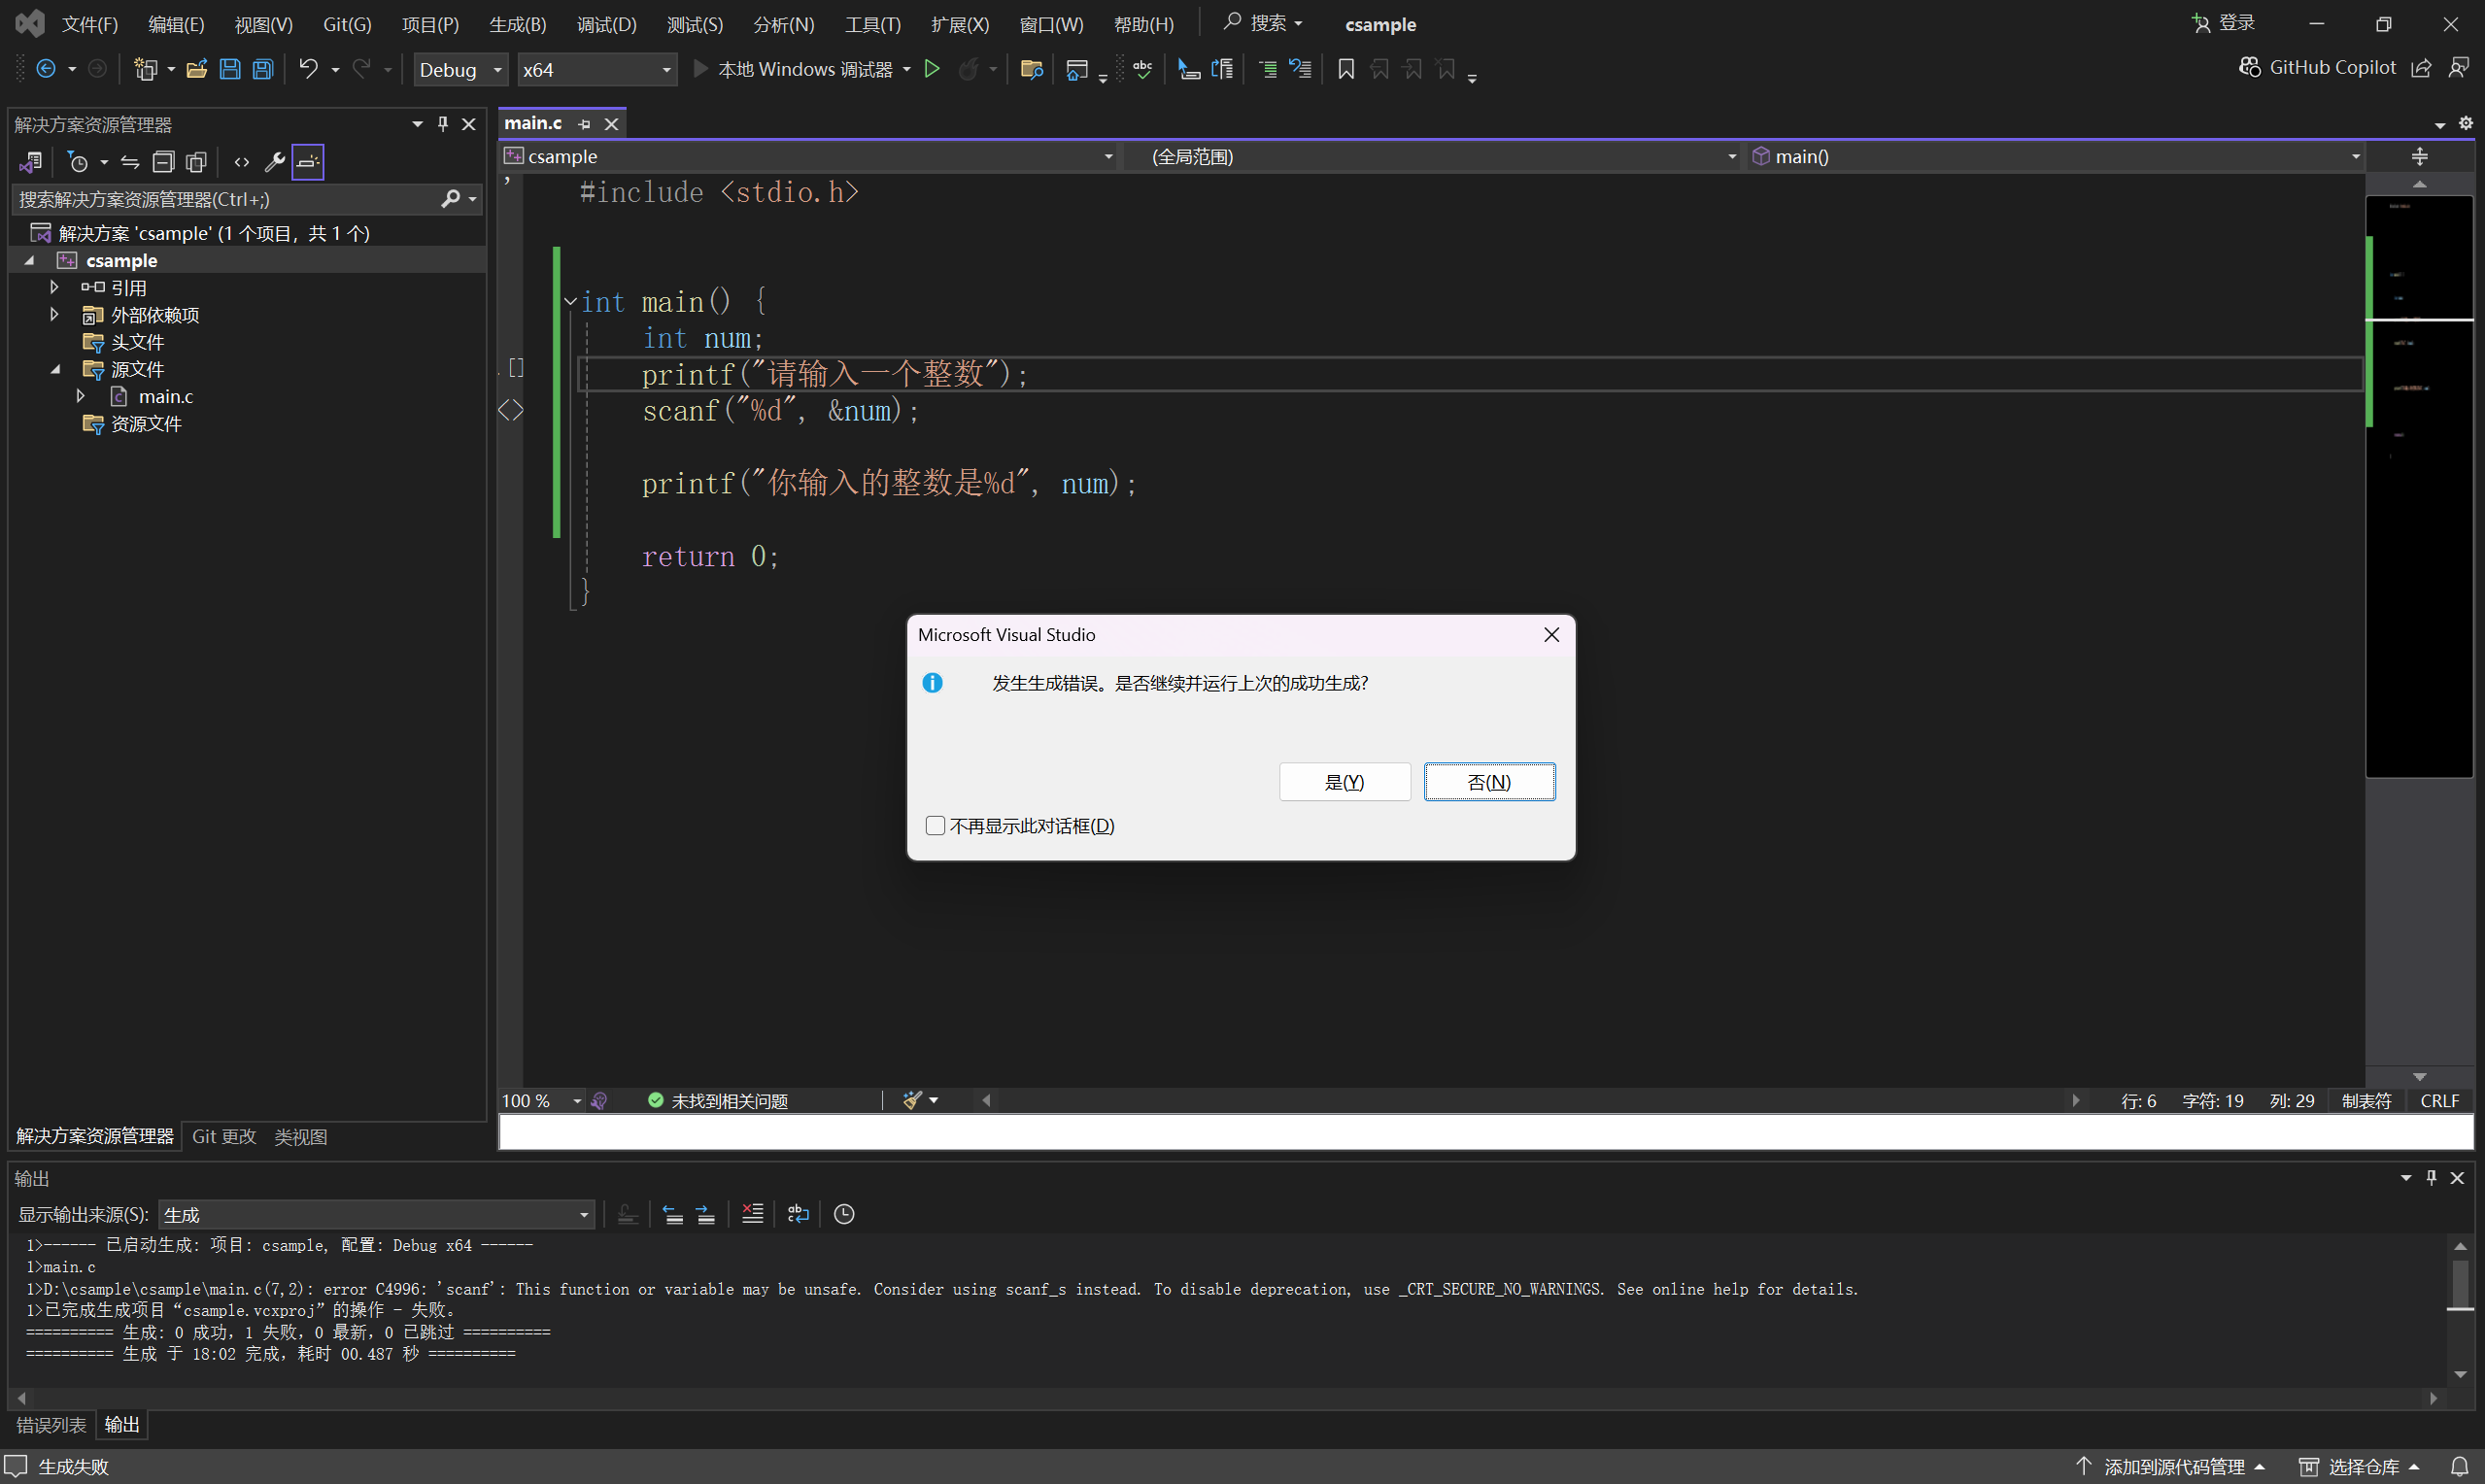
\includegraphics[width=0.8\textwidth, height=0.4\textheight]{images/1标准输入报错.png}
\end{figure}

这个窗口的意思是我们的代码有问题,过不了编译。在实际编程开发时,由于我们很难做到一次就尽善尽美,所以常常会遇到这个窗口。还好代码的试错成本是很低的,我们只需要着手去修补自己的代码即可。我们点击否,注意到visual stdio最下面出现了这样的文本

\begin{figure}[H]
    \centering
    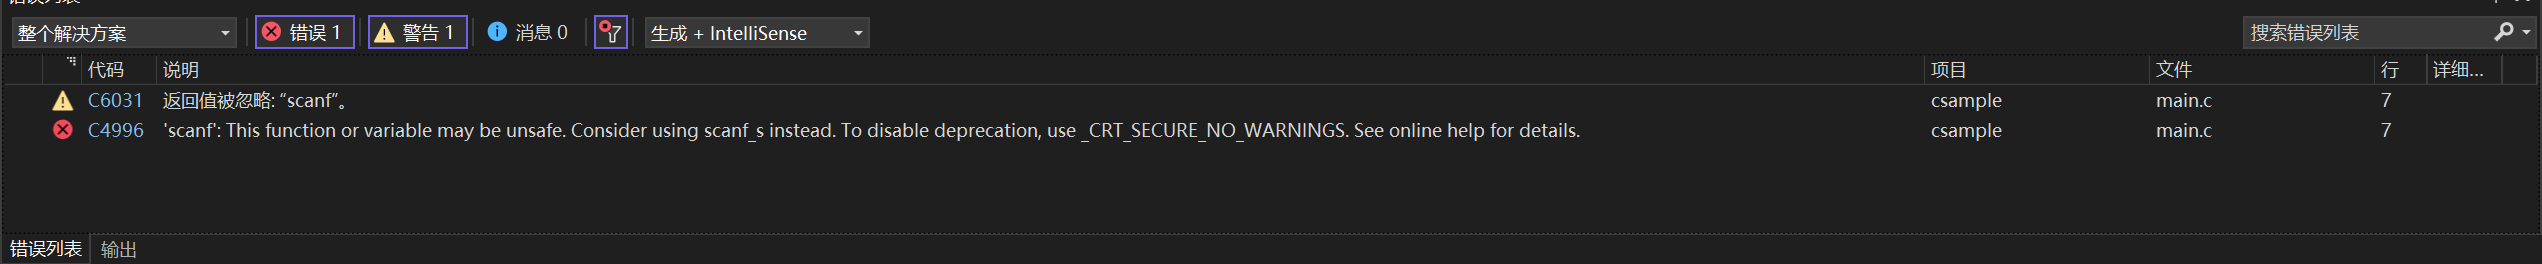
\includegraphics[width=\textwidth, height=0.2\textheight]{images/1ide错误提示.png}
\end{figure}

带有黄色警示标志的叫做警告(warning),它的意义是代码可能有一些不符合规范的地方,需要修改,但是不改也能运行。而红色标志的叫做错误(error),它的意义是这里的代码完全有问题,过不了编译,程序运行不了。我们必须要消除代码中所有的error,也要尽可能消除所有的warning。

我们开始着手消灭这个error,它的提示信息说“This function or variable may be unsafe. Consider using scanf\_s instead. To disable deprecation, use \_CRT\_SECURE\_NO\_WARNINGS. See online help for details.”

翻译成中文,就是“这个函数或者变量可能不安全。考虑使用scanf\_s替代。若要取消废弃(检查),使用\_CRT\_SECURE\_NO\_WARNINGS。详细信息见在线帮助。”。它的意思就是说,我们用的这个scanf函数不安全,已经废弃了,要么我们换用scanf\_s,要么我们加上\_CRT\_SECURE\_NO\_WARNINGS来强行使用废弃的函数。

实际上,scanf由于设计不当,会有缓冲区溢出(buffer overflow)的风险,所以我们确实不应该使用它。但是呢,只有我们使用的visual stdio会报这个错误,其它ide不会强制要求你换,而且大部分的c语言试题和c语言教程仍在使用scanf,所以我们采取强制使用废弃函数的方法来消除这个error。

在visual stdio的项目右键,点击属性,点击“C/C++”,点击“预处理器”,点击“预处理器定义”,随后点击右边出现的小箭头,点击“<编辑>”,单独一行输入“\_CRT\_SECURE\_NO\_WARNINGS”,点击“确定”即可。

此时我们再运行代码,终端首先变成这样

\begin{figure}[H]
    \centering
    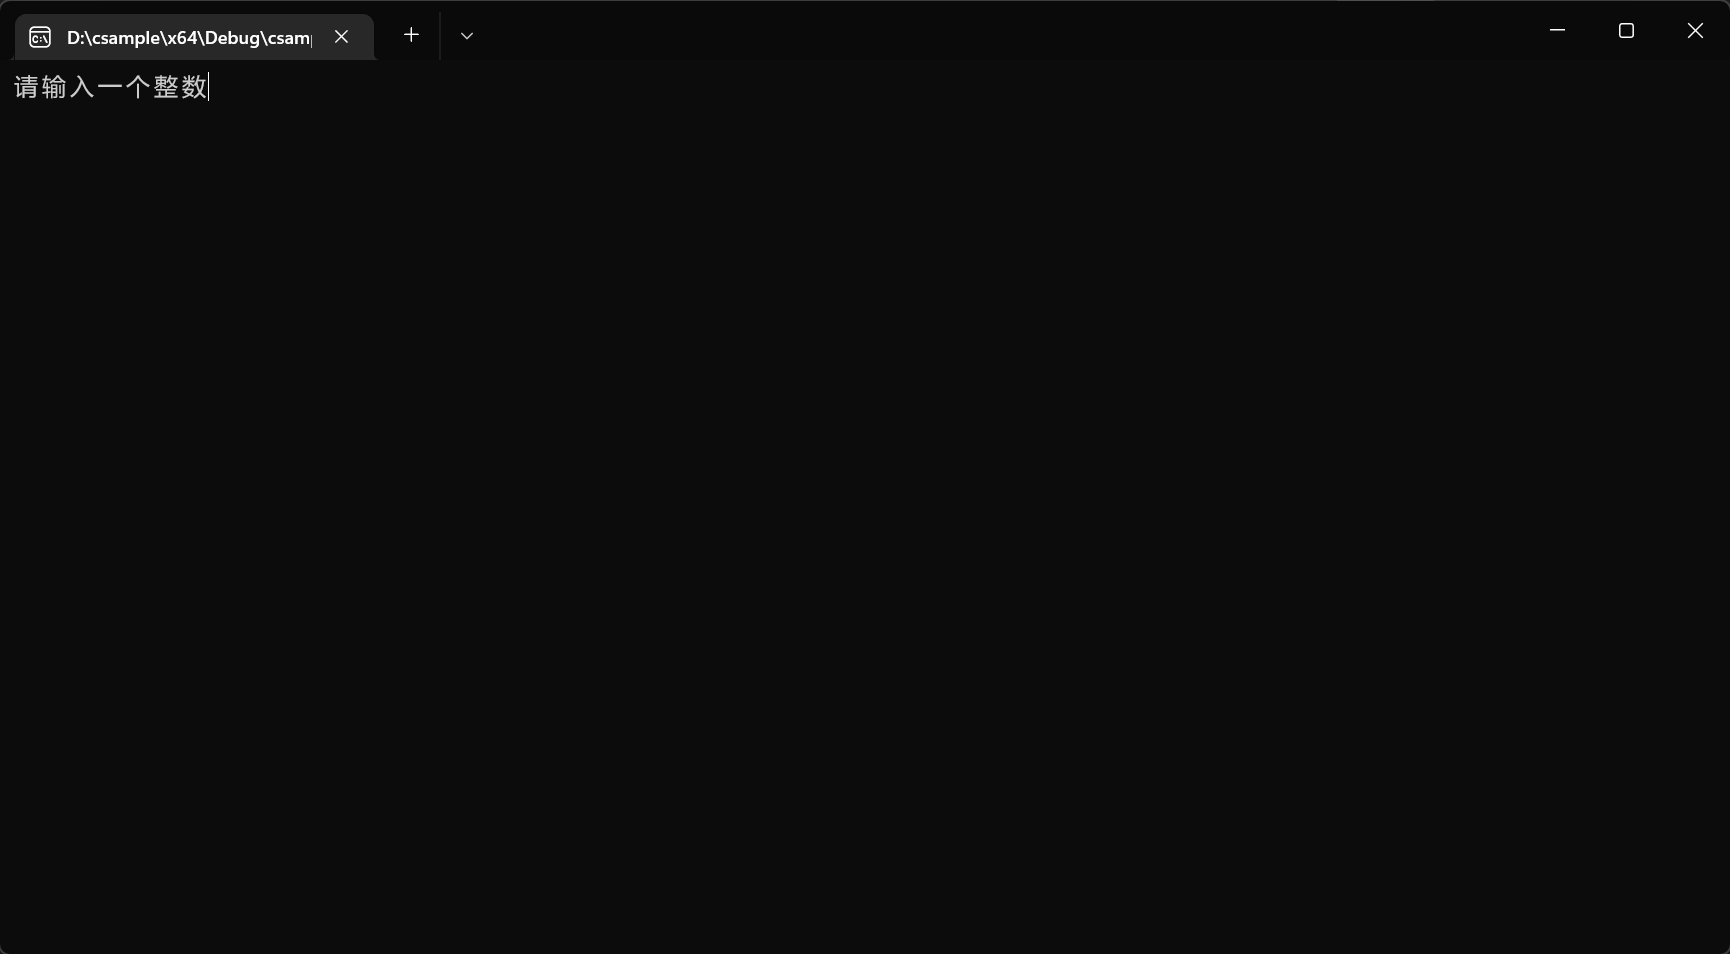
\includegraphics[width=0.8\textwidth, height=0.3\textheight]{images/1scanf首次.png}
\end{figure}

此时我们输入一个数字,点击回车,出现了这样的效果

\begin{figure}[H]
    \centering
    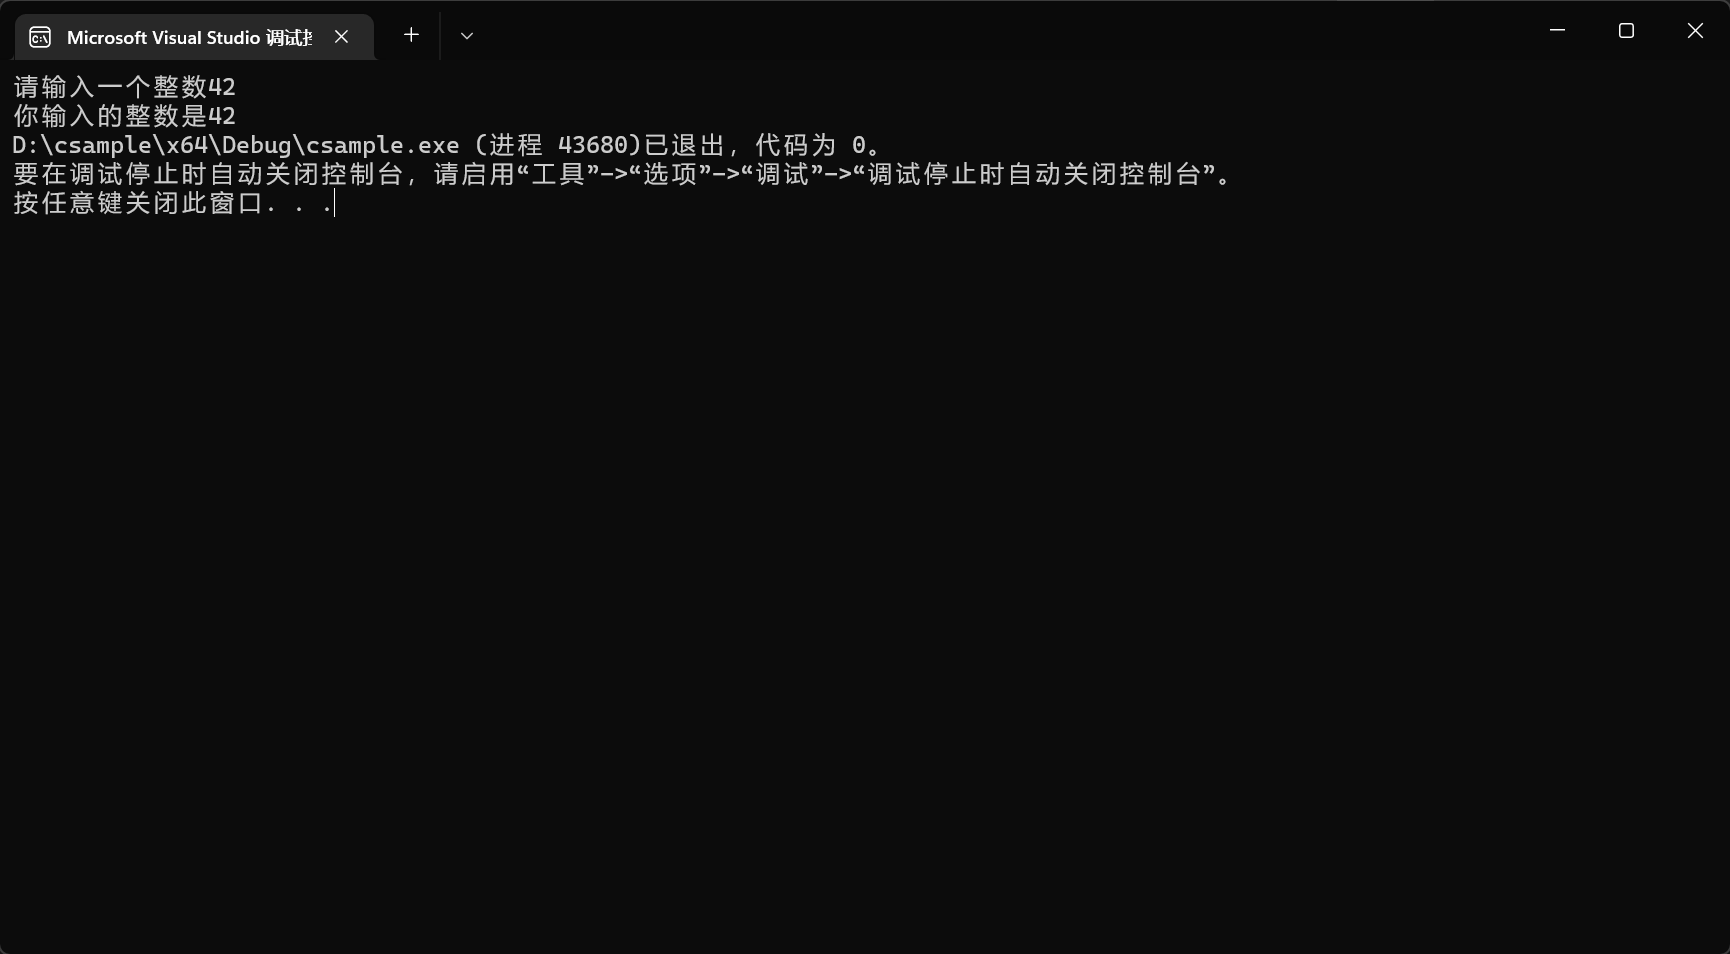
\includegraphics[width=0.8\textwidth, height=0.3\textheight]{images/1scanf完成.png}
\end{figure}

如果我们要进行的是更复杂的输入呢?比如,我们需要数学、语文和英语三科成绩,那么可以这样写

\begin{lstlisting}[language=C]
    #include <stdio.h>

    int main() {
        int math_grade;
        int chinese_grade;
        int english_grade;

        printf("请输入数学、语文、英语成绩");
        scanf("%d %d %d", &math_grade, &chinese_grade, &english_grade);

        printf("三科成绩分别是:%d, %d, %d", math_grade, chinese_grade, english_grade);
        
        return 0;
    } 
\end{lstlisting}

我们只需要按照这样输入:120 130 140,就能输出正确的成绩了。如果我们希望输入是120,130,140,那么就把scanf的一行改成

\begin{lstlisting}[language=C]
    scanf("%d,%d,%d", &math_grade, &chinese_grade, &english_grade);
\end{lstlisting}

这样我们就找到了规律,scanf的引号内的部分就像是一个模板,只有输入与模板对应,函数才正常运行。不信的话,我们可以试试在修改后的代码输入120 130 140,会得到这样的结果

\begin{figure}[H]
    \centering
    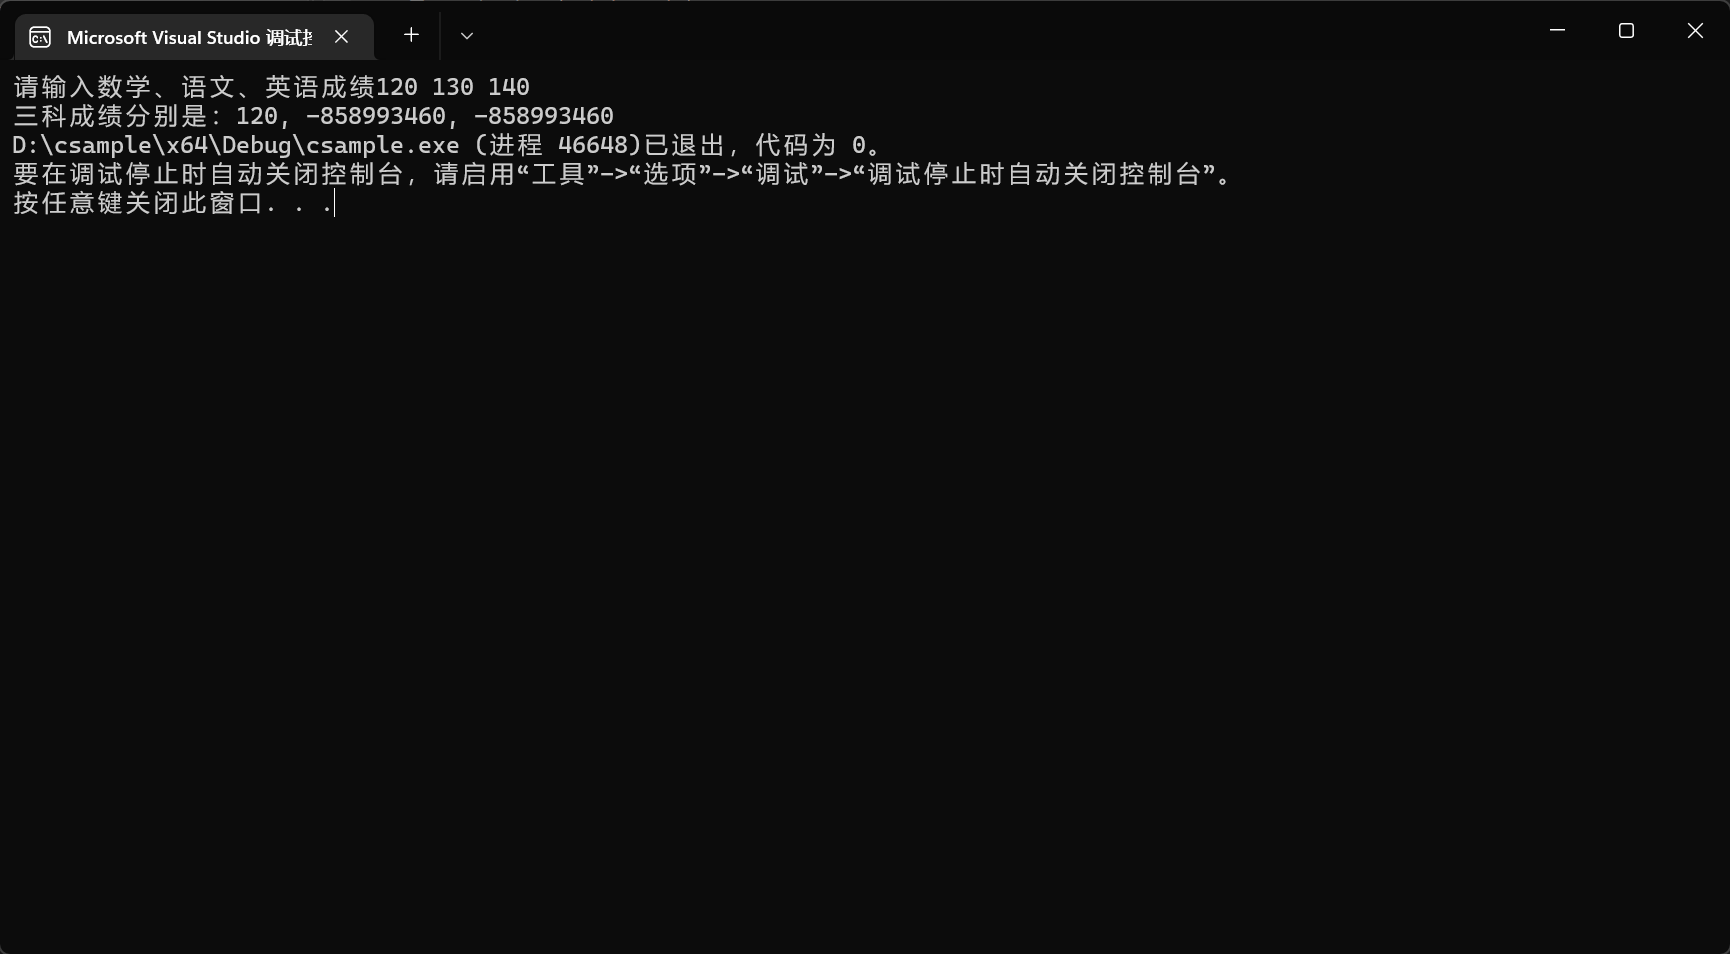
\includegraphics[width=0.8\textwidth, height=0.3\textheight]{images/1scanf出错.png}
\end{figure}

非常抽象是不是?你知道更抽象的是什么吗?假如我们使用其它编译器,那么会得到不同的结果\footnote{类似的一段代码,以120 130 140作为输入,64位电脑,处理器intel ultra9,在win11,msvc编译下运行结果为120, -858993460, -858993460;ubuntu,gcc编译下结果为120, 4096, 0;ubuntu,clang编译下结果为120, 0, 4096}。这是因为我们的输入没有符合模板的需求,模板需要我们在每两个成绩间使用英语逗号分割,我们用的却是空格,这种情况被称作未定义行为(undefined behavior),这是c语言中比较难以预测的一种的错误,我们后续会详细讲解。不知道各位记不记得,我们在解决那个error时,留了个warning尚未处理?它说我们没有使用scanf的返回值,这个“返回值”就是用来解决这个问题的,我们学习到函数时会专门提到。

\section{基本数据类型和数值运算}

\subsection{基本数据类型}

我们在上一章介绍变量的时候就已经使用了代表整数的int,但是只有整数显然是远远不够用的,c语言还提供了不同取值范围的整数、小数、字符和字符串。这些统称为基本数据类型。

在计算机科学中,整数一般被称作整型。根据取值范围的不同,总共有四种整型:short(短整型),int(整型),long(长整型)和long long,可以这样声明整型变量

\begin{lstlisting}[language=C]
    short a = 1;
    int b = 2;
    long c = 3;
    long long d = 4;
\end{lstlisting}

short的取值范围是$[-32768, 32767]$\footnote{以笔者电脑(64位win11,MSVC STL)的limits.h作为标准},int的取值范围是$[-327682147483648, 327672147483647]$,long和long long的就更大了。实际上还有一类无符号整型,就是只有非负数的整型。在整型前加一个unsigned就是对应的无符号整型

\begin{lstlisting}[language=C]
    // 无符号类型
    unsigned short a = 1;
    unsigned int b = 2;
    unsigned long c = 3;
    unsigned long long d = 4;
\end{lstlisting}

short的范围是$[-32768, 32767]$,而unsigned short的范围是$[0, 65535]$,相当于把负数部分都转移给正数了。其它类型对应的无符号类型也是一样。

介绍了这么多,笔者建议大家:除非你有明确的设计要求,对计算机了解比较清晰,非常清楚自己在写什么,否则就一律使用int。哪怕是明确了需要处理的数据都是非负也不要用无符号,哪怕是确定short就够包含自己需要的数据也要用int。

为什么我们这么说?首先,为什么c语言设计了这么多种整型和无符号这些东西呢?我们知道,在c语言诞生的年代,内存是十分紧张的资源,所以设计多种占用不同内存大小的整型也是便于程序员精准控制内存。但是现代计算机内存大多都是8GB,16GB甚至更高,已经没有必要过于珍惜内存了。

如果我们使用推荐外的类型,一方面会增大开发难度,另一方面容易诞生意料以外的问题。为什么呢?首先请考虑一个问题,以short为例,它的最大值是32767,那假如我们给一个short变量赋值32768会怎么样?我们写一段代码试一下

\begin{lstlisting}[language=C]
    #include <stdio.h>
    #include <limits.h>

    int main() {
        short a = SHRT_MAX + 1;  // SHRT_MAX就是short的最大值,即32767
        printf("%hd\n", a);
        
        return 0;
    } 
\end{lstlisting}

运行结果是-32768,也就是说,如果我们赋的值超过了数据类型取值范围的最大值,它就会从最小值开始赋。一样的,若我们赋的小于范围最小值,就会从最大值开始赋。这就像是把取值范围这根数轴首尾连接在了一起一样。类似的结果也会出现在其它类型,这是c语言的特殊设计。

想象一下,假如你在设计一个学生管理软件,为了节省内存,使用short来记录学生的编号(因为你觉得学校小,不可能超过三万人),但是使用你开发的系统的学校今年突然人数暴增,现在学校内有了32768人,那么最后一个同学的编号就是-32768,这位同学得有多无奈?因此,一般不要使用比int小的类型的。

既然使用short有这样的危害,为什么不都使用long呢?首先,实际场景中很少存在数据大到连int都装不下的情况(谁家学校有三百多亿人啊),因此没必要选这么大的;另一方面,如果需要处理的数据都是普遍极大的,一般都是由开发者自行实现适用的记录长数字的类型,使用long不划算。所以我们也一般不考虑比int大的类型。

那么为什么无论使用场景都不用无符号呢?首先,无符号的最大值和最小值也是连接在一起的,这种情况更刺激:假如一个学校有65536名学生,我们使用unsigned short来编号,那么最后一位和第一位的编号是一样的,就没办法区分这二人了。其次,我们有时设计的一些复杂算法可能出错,若算法应只输出正值却输出了负值,那么说明算法一定出了问题,假如我们使用无符号类型,就无法这样判断了。

为什么不同整型有不同取值范围呢?这实际上与其占用的比特数有关。c语言提供了sizeof运算符,用于获取一个数据类型占用的比特数(比特数是一个整型)。比如,我们可以这样获取int所占用的比特数

\begin{lstlisting}[language=C]
    #include <stdio.h>

    int main() {
        int s = sizeof(int);
        printf("%zd\n", s);
        
        return 0;
    } 
\end{lstlisting}

输出结果是4。类似的我们可以知道其它整型的大小

\begin{lstlisting}[language=C]
    #include <stdio.h>

    int main() {
        printf("%zd\n", sizeof(short));
        printf("%zd\n", sizeof(int));
        printf("%zd\n", sizeof(long));
        printf("%zd\n", sizeof(long long));

        printf("%zd\n", sizeof(unsigned short));
        printf("%zd\n", sizeof(unsigned int));
        printf("%zd\n", sizeof(unsigned long));
        printf("%zd\n", sizeof(unsigned long long));
        
        return 0;
    }
\end{lstlisting}

我们发现,占用比特数越大,储存数字的范围越大。这是一个定性的结果,我们在更深层次的课程会详细解释储存数据的原理、取值范围如何计算。

小数在计算机科学一般称作浮点型,常用的是double(双精度浮点型),还有一种叫做float,这个用法与double一致,但是我们推荐使用double。我们可以这样定义一个浮点型变量

\begin{lstlisting}[language=C]
    double a = 1.23;  // 小数点是英文句号
\end{lstlisting}

如何打印浮点数呢?打印double的占位符是\%lf,打印float的占位符是\%f,比如

\begin{lstlisting}[language=C]
    #include <stdio.h>

    int main() {
        double a = 3.14;
        printf("%lf\n", a);
        
        return 0;
    }
\end{lstlisting}

输出结果是3.140000。默认的\%lf为我们保留了六位小数,如果我们把a改成3.1415926,输出结果是3.141593,不仅保留了六位小数,还做了四舍五入。实际上,\%f也可以用在打印double上,但是使用scanf时就必须要用\%lf了。因此我们推荐在处理double时不要混用,一律使用\%lf。

如果小数太长,我们只需要显示前两位,我们就可以这样使用占位符

\begin{lstlisting}[language=C]
    printf("%.2lf\n", a);
\end{lstlisting}

它的意思是要保留小数点后两位数字,还是很形象的吧?假如我们这么写,并且把a的值改成3.14

\begin{lstlisting}[language=C]
    printf("%5.2lf\n", a);
\end{lstlisting}

输出就变成了“ 3.14”,注意多出一个空格。对于\%a.bf和\%a.blf,小数点之前的数字代表最少要输出多少位(注意小数点也算一位),之后的数字代表要输出多少位小数。如果要求最少输出位数比数字本身有的位数还多,那就会在最前面输出空格来补齐差距。

还记得字面量吗?数字42是字面量,更具体地说,它是整型字面量;数字3.14是浮点型字面量;“xyz”是字符串字面量(字符串在后续讲到)。总之,字面量可以更精确地描述为类型+字面量。

整型和浮点型都具有加减乘除四种数值运算,整型还有取模运算。一个整型可以与另一个整型做数值运算,也可以与一个整型字面量数值运算,两个整型字面量也可以进行运算。加减乘除的符号分别是$+-*/$,就像数学的写法一样,在运算符两边写参与运算的数字。像是算一加一就是$1+1$,算二乘二就是$2*2$。另外需要特别说明,赋值号只在赋值号右边的运算都完成后才会把右边的值赋给左边。举个例子

\begin{lstlisting}[language=C]
    #include <stdio.h>

    int main() {
        int a = 1;  // a和b都是整型变量
        int b = 2;
        int c = a + b;  // 整型变量进行数值运算,得到的值赋给了c。注意:只有在赋值号右边的运算完成后,赋值号才进行赋值
        printf("%d\n", c);  // 输出结果是3

       	int d = 1;
        int e = d * 4;  // e由一个整型变量和整型字面量计算得到
        printf("%d\n", e);  // 输出结果是4

        int f = 2 - 2;  // f由两个整型字面量计算得到
        printf("%d\n", f);   // 输出结果是0
        
        return 0;
    }
\end{lstlisting}

最需要强调的是除法运算。整型的运算只能算出整型,所以假如参与除法运算的两个数不能整除怎么办?我们试一试

\begin{lstlisting}[language=C]
    #include <stdio.h>

    int main() {
        int a = 2;
        int b = 3;
        int c = a / b;
        printf("%d\n", c);
        
        return 0;
    }
\end{lstlisting}

照理来说,$2/3$的结果是0.666循环,但是这段代码的输出是0。这说明,整型的除法在无法整除的时候,会截取整数部分作为运算结果。另外考虑一个问题,以0作为除数会怎么样?0作为除数是没有意义的,在c语言中以0为除数的后果就会导致未定义行为。

除此以外,整型还有取模运算,也就是获取两数相除的余数。取模运算的符号是\%。比如

\begin{lstlisting}[language=C]
    #include <stdio.h>

    int main() {
        int a = 20;
        int b = 3;
        int c = a % b;
        printf("%d\n", c);
        
        return 0;
    }
\end{lstlisting}

输出结果是2,说明20/3的结果余2。这个运算非常重要,比如我们可以通过一个数与2的余数是否为0来判断这个数是否为偶数:如果余数为0,说明这个数能被2整除,那就是偶数,反之就是奇数。

c语言中算数是有优先级的,与数学一样,即从左到右,先算乘除后算加减,括号可以改变运算顺序。比如

\begin{lstlisting}[language=C]
    int a = 4 * 2 + 2;
	int b = 4 * (2 + 2);
\end{lstlisting}

a的值是10,b的值是16。注意,如果你需要套多层括号来改变运算顺序,都使用圆括号(即())而不要使用方括号和花括号。

我们刚刚提到了赋值号是先对右边进行运算再赋给左边,所以我们实际上可以写出这样的东西

\begin{lstlisting}[language=C]
    int a = 1;
    a = a + 1;
\end{lstlisting}

首先对右边计算,是1+1=2,随后将2赋给了a,此时a就变成2了。当然了,对于其它几种数值运算也能这样使用。

像上面这样的运算是很常用的,但是每次都写成那样岂不是很麻烦?c语言提供了一种简化语法

\begin{lstlisting}[language=C]
    int a = 1;
    a += 1;  // 等价于 a = a + 1;
    // 类似的,a *= 2就等价 a = a * 2,诸如此类
\end{lstlisting}

在后续学习到流程控制时,我们需要常常对一个整型变量进行加一或者减一的运算,此时哪怕是上面的简化语法也太累赘了,因此c语言设计了自增运算符和自减运算符,用于对整型进行加一或减一的操作(其实对浮点型也适用,不过最常用于整型)。

自增运算符和自减运算符都分为前置和后置两种

\begin{lstlisting}[language=C]
    int a = 1;
    ++a;  // 前置自增运算符
    a++;  // 后置自增运算符
    --a;  // 前置自减运算符
    a--;  // 后置自减运算符
\end{lstlisting}



\section{流程控制 选择语句}

\subsection{布尔代数基础}

我们一切命题,最终都会回到“是”与“否”的基本判断上。我们若使用1代表真,使用0代表假,便很容易得到一些逻辑运算。

首先是和关系。我们说,“我和那位同学都是女生”,这句话成立的条件是我是女生,并且那位同学也是女生。也就是说,和关系意味着两个条件都成立。

\begin{align*}
    0\quad and\quad 0 \Rightarrow 0\\
    1\quad and\quad 0 \Rightarrow 0\\
    0\quad and\quad 1 \Rightarrow 0\\
    1\quad and\quad 1 \Rightarrow 1
\end{align*}

类似地,或关系成立的条件是两个条件成立一个即可。比如“A或B是女生”,只要A与B之一是女生就成立,若都是女生也成立。

\begin{align*}
    0\quad or\quad 0 \Rightarrow 0\\
    1\quad or\quad 0 \Rightarrow 1\\
    0\quad or\quad 1 \Rightarrow 1\\
    1\quad or\quad 1 \Rightarrow 1
\end{align*}

还有一种基本的就是非关系。“我不是女生”若成立,就说明“我是女生”不成立,因此

\begin{align*}
    not\quad 0 \Rightarrow 1\\
    not\quad 1 \Rightarrow 0 
\end{align*}

使用以上三种运算,我们可以结合出很多复杂的运算。比如,“A是女生或B不是女生”,就是A是女生或者B是男生时成立。总之,这样的逻辑运算一定要能够想明白。

\subsection{if语句}

if语句用于条件判断,若判断为真,就进入下属的语句,反之就不进入。它的语法是if (表达式) 下属语句。这里的表达式将会是一个数字,如果这个数字为0就不进入,反之都进入。比如,我们可以这样写

\begin{lstlisting}[language=C]
    #include <stdio.h>

    int main() {
        int a = 1;

        if (a) printf("a的值不是0");
        printf("已经完成判断\n");

        return 0;
    }
\end{lstlisting}

输出结果是“a的值不是0已经完成判断”。因为用于判断的表达式的结果是数字1,可以进入下属语句。如果将a的值改为0,就不会进入下属语句了。

如果需要在下属语句部分写多行代码怎么办,这就需要我们使用花括号把代码括起来,就像是

\begin{lstlisting}[language=C]
    #include <stdio.h>

    int main() {
        int a = 1;

        if (a) {
            printf("a的值不是0\n");
            printf("a的值是%d\n", a);
        }
        printf("已经完成判断\n");

        return 0;
    }
\end{lstlisting}

实际上,我们推荐无论下属语句是一行还是多行,都是用花括号括起来。这样可以避免不必要的错误。

在c语言中,我们有一些用于对数字进行大小比较的运算符,它们是相等判断,不等判断和大于、小于、大于等于以及小于等于符号。我们常常在流程控制的语句中使用它们。

\begin{longtable}{c|c}
     关系 & 操作符\\
     \hline
     等于 & ==\\
     \hline
     不等 & !=\\
     \hline
     小于 & <\\
     \hline
     大于 & >\\
     \hline
     小于等于 & <=\\
     \hline
     大于等于 & >=\\
\end{longtable}

这些符号可以这样使用

\begin{lstlisting}[language=C]
    #include <stdio.h>

    int main() {
        int a = 5;
        int b;  // 储存输入的数字

        printf("输入一个数,比较其与5的大小关系!\n");
        scanf("%d", &b);

        // 判断a和b(也即预设的数字和输入的数字)大小关系
        if (a <= b) {
            printf("输入的数大于等于5\n");
        }
        if (a > b) {
            printf("输入的数小于5\n");
        }

        return 0;
    }
\end{lstlisting}

\begin{lstlisting}[language=C]
    #include <stdio.h>

    int main() {
        int a = 5;
        int b;  // 储存输入的数字
        printf("请输入一个数,猜猜和预设的是否一样\n");
        scanf("%d", &b);

        // 判断a和b(也即预设的数字和输入的数字)是否相等,如果相等就进入下属语句
        if (a == b) {
            printf("你猜对了!");
        }
        // 判断a和b(也即预设的数字和输入的数字)是否相等,如果不等就进入下属语句
        if (a != b) {
            printf("你猜错了!");
        }
        
        return 0;
    }
\end{lstlisting}

在讲取模运算符的时候,我们提到,它可以用来判断一个数字的奇偶性,我们来试试设计一个程序,输入一个整数,判断其奇偶性。

开发项目一定要按照我们之前提过的步骤进行。首先我们确定设计需求:一,输入一个整数;二,判断这个整数的奇偶性;三,根据奇偶性分别输出。第一个需求使用scanf即可,第二个使用我们学习过的取模运算符进行判断即可,第三个使用if语句就能实现。我们来编写代码。

第一个需求是比较简单的,我们直接给出代码

\begin{lstlisting}[language=C]
    #include <stdio.h>

    int main() {
        int a;
        printf("请输入一个整数\n");
        scanf("%d", &a);
        
        return 0;
    }
\end{lstlisting}

接下来就要判断奇偶性了。我们之前提到,一个数字若是偶数,那么它与2的模一定为0(因为偶数一定被2整除),因此对于输入的数字,如果与2取模的结果是0,那么就是偶数,反之就是奇数。因此我们首先写出了判断偶数的程序

\begin{lstlisting}[language=C]
    if (a % 2 == 0) {
        printf("你输入了一个偶数\n");
    }
\end{lstlisting}

那么判断奇数怎么写?仔细想想,一个数与2的余数,除了0,只能是1。因此

\begin{lstlisting}[language=C]
    if (a % 2 == 1) {
        printf("你输入了一个奇数\n");
    }
\end{lstlisting}

这样我们就完成了整个程序的设计。完整代码如下

\begin{lstlisting}[language=C]
    #include <stdio.h>

    int main() {
        int a;
        printf("请输入一个整数\n");
        scanf("%d", &a);

        if (a % 2 == 0) {
            printf("你输入了一个偶数\n");
        }
        if (a % 2 == 1) {
            printf("你输入了一个奇数\n");
        }
        
        return 0;
    }
\end{lstlisting}

上面的代码确实完成了我们的需求,但是我们发现,一个数要么是奇数,要么是偶数,我们其实只需要判断一次就能知道数的奇偶性,而不是需要像现在这样费力地构造逻辑上相反的语句。所以如果if语句可以有两个从属语句,如果条件满足就转向第一个,反之转向第二个,我们的程序就能大幅简化。c语言提供了这样的语法,就是else语句。else语句跟在if语句后,就像是

\begin{lstlisting}[language=C]
    if (a % 2 == 0) {
        printf("你输入了一个偶数\n");
    } else {
        printf("你输入了一个奇数\n");
    }
\end{lstlisting}

使用else语句改造后的代码就直观简洁多了。

我们之前提到了布尔代数,三种基本的布尔运算在c语言中也有对应的语法。

\begin{longtable}{c|c}
    布尔运算 & 符号\\
    \hline
    和运算 & \&\&\\
    \hline
    或运算 & ||\\
    \hline
    非运算 & !\\ 
\end{longtable}

比如说,我们可以这样判断一个数是否包含于$[10, 100]$的区间内。

\begin{lstlisting}[language=C]
    if (a >= 10 && a <= 100)
    // 注意,不能写成这样:if (10 <= a <= 100)
\end{lstlisting}

我们可以这样判断一个数是否同时满足不是3的倍数或是偶数

\begin{lstlisting}[language=C]
    if (a % 3 != 0 || a % 2 == 0)
\end{lstlisting}

我们之前写了这样的代码来判断一个数是否为偶数

\begin{lstlisting}[language=C]
    if (a % 2 == 0)
\end{lstlisting}

实际上,上面的式子可以改成这样

\begin{lstlisting}[language=C]
    if (!(a % 2))
\end{lstlisting}

这是在干什么?最内层括号计算了a与2的余数,如果a是偶数,那么得到的结果就是0,我们想要进入下属语句,因此把运算结果使用非运算反过来就可以了。一样的,如果我们输入的是奇数,得到的结果是1,非运算后就变成了0,就不会进入下属语句了。因此,我们将判断奇偶数改成了一种更加简洁的语法。注意不要遗漏了取模运算的括号,否则非运算先与a结合,就得不到我们期望的结果了。

有了布尔代数的知识,我们可以解决一类更复杂的问题。比如,给定一个成绩,要判断它属于不及格($[0, 60)$),及格($[60, 80)$),良好($[80, 90)$)还是优秀($[90, 100]$),我们怎么写呢?最开始的想法是这样的

\begin{lstlisting}[language=C]
    #include <stdio.h>

    int main() {
        int a;
        printf("请输入成绩\n");
        scanf("%d", &a);

        if (a >= 0 && a < 60) {
            printf("未及格!\n");
        }
        if (a >= 60 && a < 80) {
            printf("及格!\n");
        }
        if (a >= 80 && a < 90) {
            printf("良好!\n");
        }
        if (a >= 90 && a <= 100) {
            printf("优秀!\n");
        }
        
        return 0;
    }
\end{lstlisting}

这样有三个问题:一,假如输入的数字大于100,或者小于0怎么办?我们还需要写一个if来捕获这种情况;二,我们的程序是按照顺序执行的,比方说我们输入的数字是65,在第二个if已经捕获了,照理来说就不需要再去判断下面的几个if了,但是它还是会执行下去,这样浪费了很多性能;三,这一系列的if逻辑上是连续的,但是我们的代码表现出来是孤立的,这样增大了阅读难度。

怎么解决呢?c语言提供了else if语句,我们将上面的代码改成

\begin{lstlisting}[language=C]
    if (a >= 0 && a < 60) {
        printf("未及格!\n");
    }
    else if (a >= 60 && a < 80) {
        printf("及格!\n");
    }
    else if (a >= 80 && a < 90) {
        printf("良好!\n");
    }
    else if (a >= 90 && a <= 100) {
        printf("优秀!\n");
    }
    else {
        printf("输入数据有误\n");
    }
\end{lstlisting}

这样解决了我们提到的三个问题。else if按照从上到下的顺序执行,如果第一个if没有匹配到,就转到下一个if,直到匹配到为止。匹配到之后就执行匹配到的if的下属语句,而不会继续执行if语句。此外,我们还可以在最后缀一个else语句来处理缺省情况。

c语言提供了一个特殊的运算符,叫做三目运算符,用来快速给变量赋值。比如

\begin{lstlisting}[language=C]
    int a = b > 0 ? 4 : 5;
\end{lstlisting}

此处的英文问号和后面的英文冒号就是三目运算符了。它的含义是,当问号前的语句成立时,就使用冒号前的值,反之使用冒号后的。在我们的例子中,如果b>0是成立的,就使用冒号前的值,a的值就是4,如果b>0是不成立的,那么a就取5。这个运算符适用于上面例子中的这种简单场景,不要滥用,否则会增大代码的阅读难度。

流程控制语句是可以嵌套的,比如

\begin{lstlisting}[language=C]
    if (a > 0) {
        if (a % 2 == 0) {
            printf("a是一个大于0的偶数\n");
        } else {
            printf("a是一个大于0的奇数\n");
        }
    }
\end{lstlisting}

在嵌套时,else语句总是和与其最近的if语句匹配,这点我们观察大括号的嵌套也能看出来。我们在之后的学习和开发实战中会经常用到流程控制语句的嵌套。

最后,c语言还提供了一种switch语句,类似于if else,因为这个东西基本没用,我们就不过多介绍了。

\section{流程控制 循环语句}

\subsection{while语句}

我们经常遇到这样的场景:需要一直做某个任务直到达到某个条件为止。在c语言中就有这样的设计,即循环语句。第一种循环是while语句,它的语法是while (条件) 下属语句。如果条件满足,就进入下属语句,下属语句执行完后程序会重新判断条件,如果还满足就再进入下属语句,直到条件不再满足为止。比如,我们若想要打印1到100,就可以这样做

\begin{lstlisting}[language=C]
    #include <stdio.h>

    int main() {
        int a = 1;
        while (a <= 100) {
            printf("%d\n", a);
        }

        return 0;
    }
\end{lstlisting}

我们首先定义了一个变量a为1,随后定义了一个循环语句,它打印a的值,直到a为100为止。这样,当a小于等于100时,下属语句就会一直执行,输出a的值,当a达到100后,循环退出,程序结束。看上去很完美不是?但是,假如我们运行这段代码(不建议大家尝试),你会发现电脑一直在输出1(有些电脑甚至会卡死)。

这是为什么?仔细想想,我们发现在循环的过程中,a的值始终是1,没有增长过,因此循环一直在执行而不会终止。所以,我们要在循环里加一条语句来使a增长。while语句改成了

\begin{lstlisting}[language=C]
    while (a <= 100) {
        printf("%d\n", a);
        ++a;
    }
\end{lstlisting}

再次运行,这次结果正确了。

我们说,流程控制语句是可以嵌套的,我们可以把if和while语句嵌套在一起,比如,可以这样输出1到100之间的全部偶数

\begin{lstlisting}[language=C]
    #include <stdio.h>

    int main() {
        int a = 1;
        while (a <= 100) {
            if (a % 2 == 0) {
                printf("%d\n", a);
            }
            ++a;
        }
        
        return 0;
    }
\end{lstlisting}

我们发现,我们为了循环而特意声明的变量a就像是一个计数器一样。实际上大部分时候这个变量的作用就是充当计数器,控制循环的进行。写计数器的时候一定不要忘记它的自增。这种充当计数器的变量一般命名为i、j和k。如果你在同一段代码内需要超过三个计数器,那么应该考虑是否要简化循环。

c语言提供了continue和break关键字,前者可以退出一次循环,后者用于直接退出整个循环。比如,上面的例子可以改写成

\begin{lstlisting}[language=C]
    #include <stdio.h>

    int main() {
        int a = 1;
        while (a <= 100) {
            if (a % 2 != 0) {
                ++a;
                continue;
            }
            printf("%d\n", a);
            ++a;
        }
        
        return 0;
    }
\end{lstlisting}

这是什么意思呢?每次在while下属语句时,都会首先判断a是不是奇数,如果是就进入if的下属语句,a自增,随后退出本次循环,因此下面的printf是不会被执行的。

再比如,假如我们有一个需求:输出一个数字,打印从1到这个数字之间的所有数字,如果打印到9就不再打印,那么就可以这样写

\begin{lstlisting}[language=C]
    #include <stdio.h>

    int main() {
        int a = 1;
        int b;
        printf("请输入一个大于1的整数\n");
        scanf("%d", &b);

        while (a <= b) {
            if (a == 9) {
                break;
            }
            
            printf("%d\n", a);
            ++a;
        }
        
        return 0;
    }
\end{lstlisting}

在循环的过程中,如果a增长到了9,就会进入if的下属语句,从而退出循环。这两个例子其实并没有体现出continue和break的真正作用,我们在之后的实战学习中会领略到这二者的真正作用。

值得注意的是,如果我们嵌套了多层循环语句,那么continue和break作用于最内层的循环。我们在学习到复杂嵌套时,各位可以自行验证这个结论。

有了循环的知识,我们就可以试着编写一个程序,它可以不间断地接受输入,直到输入了某个特定的退出符号为止。比如,我们可以编写一个程序来计算若干个正整数的平均数,如果输入非正数就退出循环。

为了实现这个程序,我们还是要遵循设计程序的三个步骤。首先确定需求:一,程序要能够不间断地输入,我们可以考虑使用while语句

\begin{lstlisting}[language=C]
    while (条件) {
        scanf("%d", &a);
    }
\end{lstlisting}

现在出现了两个问题:第一,while的条件应该是什么?第二,如果把输入结果存放在一个变量里,那么下一次的结果不就覆盖上一次的了?

第一个问题实际上就是我们的第二个需求,也即输入到非正数就退出,我们可以使用break语句,把程序写成这样

\begin{lstlisting}[language=C]
    while (条件) {
        scanf("%d", &a);
        if (a <= 0) {
            break;
        }
    }
\end{lstlisting}

如果这样,我们就不需要为循环设置条件了,因为我们的退出条件写在了循环内,所以代码就改成了

\begin{lstlisting}[language=C]
    while (1) {
        scanf("%d", &a);
        if (a <= 0) {
            break;
        }
    }
\end{lstlisting}

条件是1,意味着永远成立,因此这个循环如果内层没有退出条件的话,它会永远执行下去(也就是所谓的死循环)。第二个问题的解决其实很简单,反正我们最终的目的是要求和,我们可以这样写

\begin{lstlisting}[language=C]
    int sum = 0;
    int a;

    while (1) {
        scanf("%d", &a);
        if (a <= 0) {
            break;
        }
        sum += a;
    }
\end{lstlisting}

什么意思?我们每次输入的数字,都会被加到这个变量sum中,这样,我们最终得到的就是所有输入的数字的和了。为什么这行求和要写到if语句后,而不是写成一个else语句呢?也就是这样

\begin{lstlisting}[language=C]
    while (1) {
        scanf("%d", &a);
        if (a <= 0) {
            break;
        } else {
            sum += a;
        }
    }
\end{lstlisting}

这样当然也是可以的,它意味着:如果进入if的下属语句,就不会进入else的,反之如果进入else的下属语句就进入不了if的,这符合我们的需求。但是我们发现,在修改前的代码,假如进入if的下属语句就会退出循环,也执行不到求和的那一行,假如进入了求和的一行,就说明一定没有进入if,因此效果是一样的。

像上面这样,如果添加else语句与否的执行效果相同,我们建议不要使用else,这样就减少了嵌套的数量,增加了代码的可读性。因为,我们如果阅读的是这样一段代码

\begin{lstlisting}[language=C]
    if (a <= 0) {
        break;
    } else {
        sum += a;
    }
\end{lstlisting}

我们在阅读else下的代码时就要时刻惦记着:这是if语句的另一个情况,它代表了a是大于零的。我们每次都要想着if语句的条件才能对else的代码有正确的理解。但是如果写成这样

\begin{lstlisting}[language=C]
    if (a <= 0) {
        break;
    }
    sum += a;
\end{lstlisting}

我们就可以理解为:a小于等于零的情况在前面已经处理过了,我们断定下面的代码中a是大于零的,这段if语句就像是一个卫兵,向我们保证后面代码中a的取值范围,因此这样的,在核心业务逻辑代码前用来处理异常情况的代码被称做卫语句。这样就减少了阅读时的负担,这对于修改代码和理解代码都非常重要。实际上,我们一般推荐嵌套不要超过三层,我们在后期会讲到如何减少嵌套的数量。

如果不这么写呢?我们可以通过使用while的条件来控制循环的退出。即代码改成

\begin{lstlisting}[language=C]
    while (scanf("%d", &a), a > 0) {
        sum += a;
    }
\end{lstlisting}

这是什么意思?这段代码的核心是while括号内的那一行,这里涉及到了一个叫做逗号运算符的知识,即,在作为流程控制语句条件的语句里,我们可以用逗号连接几个语句,这几个语句依次执行,但是只有最后一个作为条件判断。就拿我们这段代码来说,我们使用逗号连接了scanf和a的大小判断。首先执行scanf,将输入的值赋给a,然后执行大小判断,因为这是最后一个语句,它的判断结果就作为while的条件判断了。逗号运算符是c语言一个很实用的知识,可以在不失去阅读性的情况下简化我们的代码。当然,我们一般不会在这里连接多个语句,一般就是像上面这样连接一个,否则代码过于臃肿。

现在我们有了所有数的总和,接下来要求平均值,这就需要我们知道具体有几个数,所以我们应该定义一个变量用来储存已经求了几个数的和。那么它应该写在哪里呢?我们记录的数的个数,是用来求和的数的个数,因此应该和求和写在一块,也就是

\begin{lstlisting}[language=C]
    int sum = 0;
    int count = 0;
    int a;

    while (1) {
        scanf("%d", &a);
        if (a <= 0) {
            break;
        }
        sum += a;
        ++count;
    }
\end{lstlisting}

或者使用逗号运算符的写法

\begin{lstlisting}[language=C]
    int sum = 0;
    int count = 0;
    int a;

    while (scanf("%d", &a), a > 0) {
        sum += a;
        ++count;
    }
\end{lstlisting}

最后就要计算并打印平均数了。别忘了,整数的平均值可以是小数,所以我们要定义一个浮点型来储存结果。另外,要先把sum转成浮点型再计算,这在之前就已经讲过原因了。因此,我们最终的程序是

\begin{lstlisting}[language=C]
    #include <stdio.h>

    int main() {
        int sum = 0;
        int a;
        int count = 0;

        while (scanf("%d", &a), a > 0) {
            sum += a;
            ++count;
        }

        double re = (double) sum / count;
        printf("%lf\n", re);
        
        return 0;
    }
\end{lstlisting}

当然了,如果是我们自己使用,那么可以增添一些提示性的文本,比如

\begin{lstlisting}[language=C]
    #include <stdio.h>

    int main() {
        int sum = 0;
        int a;
        int count = 0;

        printf("请输入连续若干个正整数,每输入一个就按一次回车。输入非正整数表示输入完成\n");

        while (scanf("%d", &a), a > 0) {
            sum += a;
            ++count;
        }

        double re = (double) sum / count;
        printf("以上数字的平均值是:%lf\n", re);
        
        return 0;
    }
\end{lstlisting}

其实c语言提供了一种类似于while的语句,叫做do while,比如

\begin{lstlisting}[language=C]
    do {
        printf("hi\n");
    } while (a > 5);
\end{lstlisting}

与while

\begin{lstlisting}[language=C]
    while (a > 5) {
        printf("hi\n");
    }
\end{lstlisting}

区别在于,do while要先执行一次do内的语句,然后再根据while判断是否循环。也就是说,do while会至少执行一次循环内的语句,而while不一定。

我们在使用while语句解决一些需要重复若干次循环的问题时,会发现它不太方便,比如我们想要打印10次Hello World

\begin{lstlisting}[language=C]
    int i = 1;
    while (i <= 10) {
        printf("Hello World\n");
        ++i;
    }
\end{lstlisting}

我们发现,为了循环计数,我们在外层定义了一个变量,还要在循环里时刻想着别忘了它的自增。这样非常麻烦,因此c语言提供了for语句,它的语法是 for (初始条件; 终止条件; 赋值语句) 下属语句。比如上面的例子,我们可以这样使用for语句实现

\begin{lstlisting}[language=C]
    for (int i = 0; i < 10; ++i) {
        printf("Hello World\n");
    }
\end{lstlisting}

这是什么意思呢?在执行for语句的时候,首先执行初始条件,创建了一个叫做i的变量,随后执行终止条件,发现满足,因此执行下属语句。下属语句执行完了,就会执行赋值语句,随后再执行终止条件。如果仍满足条件就继续执行下属语句,然后再执行赋值语句,如此一直循环,直到不满足终止条件为止,此时退出循环。

在我们的示例中,我们首先创建了变量i,然后到了终止条件,发现满足i小于10,因此执行下属语句,打印了一次,随后执行赋值语句,i变成了1,一直这样执行,直到i变成了10,此时不满足终止条件了,退出循环。我们从0一直执行到9,执行了10次。

那么,为什么不像while的例子那样,写成这样

\begin{lstlisting}[language=C]
    for (int i = 1; i <= 10; ++i) {
        printf("Hello World\n");
    }
\end{lstlisting}

从1开始,这两段代码效果相同,但是后者不是更好理解吗?其实不是,计算机世界往往从0开始计数(学习指针时会解释为什么),我们这样写,还节省了一个等号,这样代码看上去反而更简洁有效。毕竟,区间$[1, 10]$内的整数个数就等于$[0, 9]$的,因此也等于$[0, 10)$的。

就是说,如果我们想要重复n次,那么代码就写成

\begin{lstlisting}[language=C]
    for (int i = 0; i < n; ++i)
\end{lstlisting}

这样的话,i就相当于一个计数器一样。值得注意的是,定义的临时变量只在for循环内有效,即

\begin{lstlisting}[language=C]
    for (int i = 0; i < n; ++i) {
        // 这里可以使用i
    }
    // 这里不能用i
\end{lstlisting}

在for循环的下属语句内,我们也可以改变i的值。另外for也可以使用continue和break,比如我们在while写的输出1到100内偶数的例子,使用for可以改成

\begin{lstlisting}[language=C]
    #include <stdio.h>

    int main() {
        for (int i = 1; i <= 100; ++i) {
            if (i % 2 != 0) {
                continue;
            }
            printf("%d\n", i);
        }
        
        return 0;
    }
\end{lstlisting}

为什么i又赋成1了?我们要灵活变通,i在这里不只是计数器,它还要被输出,因此这样写更好。

有意思的是,for的初始条件、终止条件和赋值语句都可以不写,而是使用别的地方的代码替代。比如,如果我们使用的是定义在别的地方的变量作为循环的变量,那么就可以这样写

\begin{lstlisting}[language=C]
    int a = 0;
    for (; a < n; ++a) {}
\end{lstlisting}

也即,我们空下了初始条件部分。如果我们退出循坏是通过下属语句的break,那么for循环就可以写成

\begin{lstlisting}[language=C]
    for (int a = 0;; ++a) {
        if (a >= n) {
            break;
        }
    }
\end{lstlisting}

再比如,如果我们对a的赋值在下属语句,那么可以不写赋值语句

\begin{lstlisting}[language=C]
    for (int a = 0; a < n;) {
        ++a;
    }
\end{lstlisting}

总之,不需要哪部分就不写哪部分即可,但是不要忘记使用分号隔开各个部分。当然了,我们还可以同时不写多个部分,这都取决于具体情况。另外,有时我们会见到这样的代码

\begin{lstlisting}[language=C]
    for (;;) {}
\end{lstlisting}

这就是一个死循环,等价于

\begin{lstlisting}[language=C]
    while (1) {}
\end{lstlisting}

我们在引入for的时候就解释了它相对于while的优势,那么while的优势是什么?我们发现,for语句更像是为了确定循环次数的情况而设计的,在不确定循环次数的情况下,while更加简单。这二者都很重要,在实际开发时要经过思考后选用合适的循环语句。


\end{document}
